\documentclass[notes,10pt, aspectratio=169]{beamer}

\usepackage{pgfpages}
% These slides also contain speaker notes. You can print just the slides,
% just the notes, or both, depending on the setting below. Comment out the want
% you want.
% Note visibility is selected after package loading at the end of this preamble.
%\setbeameroption{show only notes} % Only notes
%\setbeameroption{show notes on second screen=right} % Both

\usepackage{helvet}
\usepackage[default]{lato}
\usepackage{array}
\usepackage{eurosym}
\usepackage{setspace}
\usepackage{animate}
\usepackage{multicol}
\usepackage{breqn}
\usepackage{subcaption}
\usepackage{caption}
\captionsetup{font=scriptsize, justification=raggedright,singlelinecheck=false}
\usepackage[export]{adjustbox}
\usepackage[scale=2]{ccicons}
\usepackage{tikz}
\newenvironment{wideitemize}{\itemize\addtolength{\itemsep}{10pt}}{\enditemize}
\usepackage{natbib}

\usepackage{tikz}
\usepackage{verbatim}
\setbeamertemplate{note page}{\pagecolor{yellow!5}\insertnote}
\usepackage{amsmath}
%\usepackage{mathpazo}
\usepackage{hyperref}
\usepackage{lipsum}
\usepackage{multimedia}
\usepackage{multirow}
\usepackage{graphicx}
\usepackage{dcolumn}
\usepackage{bbm}
\newcolumntype{d}[0]{D{.}{.}{5}}

\usepackage{changepage}
\usepackage{appendixnumberbeamer}
% \newcommand{\beginbackup}{
%   \newcounter{framenumbervorappendix}
%   \setcounter{framenumbervorappendix}{\value{framenumber}}
%   \setbeamertemplate{footline}
%   {
%      \leavevmode%
%      \hline
%      box{%
%       \begin{beamercolorbox}[wd=\paperwidth,ht=2.25ex,dp=1ex,right]{footlinecolor}%
% %         \insertframenumber  \hspace*{2ex}
%       \end{beamercolorbox}}%
%      \vskip0pt%
%   }
%  }

 \setbeamertemplate{footline}{
    \hbox{%
    \begin{beamercolorbox}[wd=\paperwidth,ht=3ex,dp=1.5ex,leftskip=2ex,rightskip=2ex]{page footer}%
        %\usebeamerfont{title in head/foot}%
        %\insertshorttitle \hfill
        %\insertsection \hfill
        %\tableofcontents[currentsection] \hfill
        \insertsectionnavigationhorizontal{0.7\paperwidth}{}{} \hfill
        \insertframenumber{} / \inserttotalframenumber
    \end{beamercolorbox}}%
}
\newcommand{\backupend}{
   \addtocounter{framenumbervorappendix}{-\value{framenumber}}
   \addtocounter{framenumber}{\value{framenumbervorappendix}}
}


\usepackage{graphicx}
\usepackage[space]{grffile}
\usepackage{booktabs}

% These are my colors -- there are many like them, but these ones are mine.
\definecolor{blue}{RGB}{0,114,178}
\definecolor{red}{RGB}{213,94,0}
\definecolor{yellow}{RGB}{240,228,66}
\definecolor{green}{RGB}{0,158,115}

\setbeamercolor{section in head/foot}{fg=blue}

\useinnertheme[shadow]{rounded}
\setbeamercolor{block title example}{fg=black,bg=orange!50!white}
\setbeamercolor{block body example}{fg=black, bg=orange!30!white}


\hypersetup{
  colorlinks=false,
  linkbordercolor = {white},
  linkcolor = {blue}
}


%% I use a beige off white for my background
\definecolor{MyBackground}{RGB}{255,253,218}

%% Uncomment this if you want to change the background color to something else
%\setbeamercolor{background canvas}{bg=MyBackground}

%% Change the bg color to adjust your transition slide background color!
\newenvironment{transitionframe}{
  \setbeamercolor{background canvas}{bg=yellow}
  \begin{frame}}{
    \end{frame}
}

\setbeamercolor{frametitle}{fg=blue}
\setbeamercolor{title}{fg=black}
%\setbeamertemplate{footline}[frame number]
\setbeamertemplate{navigation symbols}{}
\setbeamertemplate{itemize items}{-}
\setbeamercolor{itemize item}{fg=blue}
\setbeamercolor{itemize subitem}{fg=blue}
\setbeamercolor{enumerate item}{fg=blue}
\setbeamercolor{enumerate subitem}{fg=blue}
\setbeamercolor{button}{bg=white,fg=blue,}



% If you like road maps, rather than having clutter at the top, have a roadmap show up at the end of each section
% (and after your introduction)
% Uncomment this is if you want the roadmap!
% \AtBeginSection[]
% {
%    \begin{frame}
%        \frametitle{Roadmap of Talk}
%        \tableofcontents[currentsection]
%    \end{frame}
% }
\setbeamercolor{section in toc}{fg=blue}
\setbeamercolor{subsection in toc}{fg=red}
%\setbeamersize{text margin left=1em,text margin right=1em}
\setbeamersize{text margin left=0.7cm,text margin right=0.7cm}


\title[]{\textcolor{blue}{Seminar 3:}}
\subtitle{Classroom problems and worked solutions}
\author{25117 - Econometrics}
\institute[shortinst]{Universitat Pompeu Fabra}

%\date{September 25th, 2024}


% Each problem is followed by worked solution slides. Set \showsolutionsfalse
% below to compile a problem-only deck. Hidden \note entries retain instructor
% guidance. All data are hypothetical; no external assets are needed.
\newif\ifshowsolutions
\showsolutionstrue
\newcommand{\E}{\mathbb{E}}
\newcommand{\Var}{\operatorname{Var}}
\newcommand{\Cov}{\operatorname{Cov}}
\newcommand{\Corr}{\operatorname{Corr}}
\newcommand{\answerpart}[1]{\textcolor{blue}{\textbf{#1.}}\,}

\setbeameroption{hide notes} % Speaker notes hidden; worked solutions are visible.

\begin{document}

\begin{frame}[plain]
\maketitle
\end{frame}
\note{Instructor guide. This seminar follows Lecture3v2.tex: the population regression, OLS estimation and residuals, units and binary regressors, goodness of fit, assumptions and causality, population linear projection, finite-sample coefficient properties, conditional variances, and coefficient tests. All numerical examples are invented for teaching. Each problem is followed by numbered worked solutions and has a hidden instructor note. Several problems explicitly return to the same five observations so that calculations can be connected.}

\begin{frame}{The issue: what do study hours tell us about scores?}
\begin{wideitemize}
\item Fit a line to study hours and test scores, then calculate what the fitted line leaves unexplained.
\item Assess what an estimated slope says about prediction and what additional assumptions support a causal interpretation.
\item Measure the uncertainty in both coefficients and use it to test claims about the population line.
\end{wideitemize}
\begin{exampleblock}{Classroom problems}
Show the formula before substituting numbers. Worked solutions follow each problem, with answer numbers matching the subquestions.
\end{exampleblock}
\end{frame}
\note{Suggested modules: Problems 1--5 cover interpretation and OLS calculations; 6--7 cover fit and error spread; 8--10 examine population projections, confounding, and sampling; 11--14 cover unbiasedness, coefficient precision, and inference. Normal inference is used only in the explicitly large-sample Problem 14.}

\section{Model}

\begin{frame}{Problem 1: What does the population regression predict?}
In a population model, $Y$ is a student's test score in points and $X$ is weekly study time in hours, with support $X\in\{1,2,3,4,5\}$:
\[
Y=50+2X+U,\qquad \E(U\mid X)=0,
\qquad \E(Y\mid X=x)=50+2x.
\]
\begin{enumerate}
\setlength{\itemsep}{9pt}
\item Identify the outcome, regressor, intercept, and slope. State the units of the intercept and slope.
\item Calculate the conditional mean score at 2 and 4 study hours. What change in the conditional mean accompanies this change in hours?
\item A student studies 3 hours and scores 59. Find this student's realized population error. Explain why the individual score can differ from the conditional mean even though $\E(U\mid X)=0$.
\end{enumerate}
\end{frame}
\note{All numerical quantities are hypothetical teaching data. Solution to Problem 1. This population model is separate from the five-observation sample introduced in Problem 2. Y is the dependent variable in test points, X the regressor in weekly hours, beta0=50 points, and beta1=2 points per additional hour. The intercept is the line's value at x=0, which lies outside the specified support; do not describe it as an observed conditional mean at zero. Conditional means at x=2 and x=4 are 54 and 58 points. The change is beta1 times Delta X=2(4-2)=4 points. At x=3 the conditional mean is 56. The realized population error is u=59-56=3 points. Zero conditional mean restricts the average error at each x, not every realized error. The conditional regression relation alone does not establish a causal effect of study time.}

\ifshowsolutions
% SOLUTION 1 START
\begin{frame}{Solution 1: Conditional means and an individual error}
\small
\answerpart{1}$Y$ is the outcome in test points; $X$ is the regressor in weekly study hours. The intercept $\beta_0=50$ is in points and the slope $\beta_1=2$ is in points per hour. The line's intercept at $x=0$ lies outside the given support.
\par\vspace{5pt}
\answerpart{2}Using $\E(Y\mid X=x)=\beta_0+\beta_1x$,
\[
\E(Y\mid X=2)=50+2(2)=54,\quad
\E(Y\mid X=4)=50+2(4)=58.
\]
\[
\Delta\E(Y\mid X)=\beta_1\Delta x=2(4-2)=\boxed{4\text{ points}}.
\]
\answerpart{3}The realized population error is the distance from the population line:
\[
u=y-(\beta_0+\beta_1x)=59-[50+2(3)]=59-56=\boxed{3\text{ points}}.
\]
At $X=3$, the conditional mean is 56 and this student's score is 59. The condition $\E(U\mid X=3)=0$ concerns the average error among students at that value of $X$; individual errors can be positive or negative.
\end{frame}
% SOLUTION 1 END
\fi

\section{OLS}

\begin{frame}{Problem 2: Which line best fits five students?}
For a new sample, weekly study hours $X$ and test scores $Y$ are
\begin{center}
\begin{tabular}{c|rrrrr}
Student $i$ & 1 & 2 & 3 & 4 & 5 \\ \hline
$x_i$ (hours) & 1 & 2 & 3 & 4 & 5 \\
$y_i$ (points) & 52 & 54 & 53 & 58 & 58
\end{tabular}
\end{center}
\begin{enumerate}
\setlength{\itemsep}{8pt}
\item Write the OLS objective $Q(a,b)$ for a candidate line $a+bx$. Differentiate with respect to $a$ and $b$ to obtain the two first-order conditions.
\item Calculate $\overline x$, $\overline y$, and a table of $x_i-\overline x$, $y_i-\overline y$, their cross-products, and $(x_i-\overline x)^2$.
\item Derive $\widehat\beta_0=\overline y-\widehat\beta_1\overline x$ from the first condition. Calculate the OLS slope and intercept, showing why the slope also equals $s_{XY}/s_X^2$.
\end{enumerate}
\end{frame}
\note{All observations are hypothetical teaching data. Solution to Problem 2. The OLS objective is sum(yi-a-bxi) squared. Derivatives are -2 sum(yi-a-bxi) and -2 sum xi(yi-a-bxi). At the optimum, the first condition yields beta0hat=ybar-beta1hat xbar. The sample means are 3 and 55. Centered x values are -2,-1,0,1,2; centered y values are -3,-1,-2,3,3. Cross-products are 6,1,0,3,6, summing to 16. Squared centered x values are 4,1,0,1,4, summing to 10. The sample covariance is 16/4=4 hour-points, and sample x variance is 10/4=2.5 hours squared. The slope is 16/10=4/2.5=1.6 points per hour; intercept is 55-1.6(3)=50.2 points. Positive Sxx gives a unique OLS line. This sample does not use the population coefficients specified in Problem 1.}

\ifshowsolutions
% SOLUTION 2 START
\begin{frame}{Solution 2: The objective and the normal equations}
\small
\answerpart{1}For any candidate intercept $a$ and slope $b$, OLS minimizes
\[
Q(a,b)=\sum_{i=1}^n(y_i-a-bx_i)^2.
\]
Differentiating gives
\[
\frac{\partial Q}{\partial a}=-2\sum_{i=1}^n(y_i-a-bx_i),
\qquad
\frac{\partial Q}{\partial b}=-2\sum_{i=1}^n x_i(y_i-a-bx_i).
\]
At $(a,b)=(\widehat\beta_0,\widehat\beta_1)$, set both derivatives to zero:
\[
\sum_i(y_i-\widehat\beta_0-\widehat\beta_1x_i)=0,
\qquad
\sum_i x_i(y_i-\widehat\beta_0-\widehat\beta_1x_i)=0.
\]
\end{frame}

\begin{frame}{Solution 2: Centered observations and OLS coefficients (continued)}
\small
\answerpart{2}The means are
\[
\overline x=\frac1n\sum_i x_i=\frac{15}{5}=3,
\qquad
\overline y=\frac1n\sum_i y_i=\frac{275}{5}=55.
\]
\begin{center}
\begin{tabular}{c|rr|rr|rr}
$i$ & $x_i$ & $y_i$ & $x_i-\overline x$ & $y_i-\overline y$ & $(x_i-\overline x)(y_i-\overline y)$ & $(x_i-\overline x)^2$ \\ \hline
1 & 1 & 52 & $-2$ & $-3$ & 6 & 4 \\
2 & 2 & 54 & $-1$ & $-1$ & 1 & 1 \\
3 & 3 & 53 & 0 & $-2$ & 0 & 0 \\
4 & 4 & 58 & 1 & 3 & 3 & 1 \\
5 & 5 & 58 & 2 & 3 & 6 & 4 \\ \hline
Sum & 15 & 275 & 0 & 0 & 16 & 10
\end{tabular}
\end{center}
\end{frame}

\begin{frame}{Solution 2: The slope and intercept (continued)}
\small
\answerpart{3}The first normal equation implies
\[
n\overline y-n\widehat\beta_0-n\widehat\beta_1\overline x=0
\quad\Longrightarrow\quad
\boxed{\widehat\beta_0=\overline y-\widehat\beta_1\overline x}.
\]
Combining the two normal equations yields
\[
\sum_i(x_i-\overline x)(y_i-\overline y)
=\widehat\beta_1\sum_i(x_i-\overline x)^2.
\]

The common divisor $n-1$ cancels from the covariance-to-variance ratio:
\[
\widehat\beta_1
=\frac{\sum_i(x_i-\overline x)(y_i-\overline y)}{\sum_i(x_i-\overline x)^2}
=\frac{s_{XY}}{s_X^2}
=\frac{16/(5-1)}{10/(5-1)}=\frac{16}{10}=\boxed{1.6}.
\]
\[
\widehat\beta_0=\overline y-\widehat\beta_1\overline x
=55-1.6(3)=\boxed{50.2},\qquad \widehat y=50.2+1.6x.
\]
\end{frame}
% SOLUTION 2 END
\fi

\begin{frame}{Problem 3: What does OLS leave unexplained?}
Use the five observations and estimated line from Problem 2:
\[
\widehat y_i=50.2+1.6x_i.
\]
\begin{enumerate}
\setlength{\itemsep}{10pt}
\item Calculate every fitted value and residual $\widehat u_i=y_i-\widehat y_i$. Sketch the observations and fitted line, and identify a residual as a vertical distance.
\item Verify that $\sum_i\widehat u_i=0$ and $\sum_i x_i\widehat u_i=0$. Check that the fitted line passes through $(\overline x,\overline y)$.
\item Calculate the sum of squared residuals, $SSR=\sum_i\widehat u_i^2$. Compare it with the squared-error sums for the constant prediction 55 and the candidate line $50+2x$.
\end{enumerate}
\end{frame}
\note{All observations are hypothetical teaching data. Solution to Problem 3. Fitted values are 51.8,53.4,55,56.6,58.2 and residuals are .2,.6,-2,1.4,-.2. Their sum is zero. The x-weighted sum is .2+1.2-6+5.6-1=0. At xbar3 the fitted value is 55, equal to ybar. SSR=.04+.36+4+1.96+.04=6.4. The constant line55 has residuals -3,-1,-2,3,3 and squared-error sum32. The candidate50+2x has residuals0,0,-3,0,-2 and squared-error sum13. Residual orthogonality follows algebraically from fitting an intercept and slope by OLS; it does not establish a causal interpretation or zero conditional population errors. Residuals use estimated sample coefficients, whereas population errors use the unknown true coefficients. The graph's vertical axis is truncated at 50 points and labeled accordingly.}

\ifshowsolutions
% SOLUTION 3 START
\begin{frame}{Solution 3: Fitted scores and vertical residuals}
\small
\answerpart{1}Apply the fitted-value and residual formulas to each observation:
\[
\widehat y_i=\widehat\beta_0+\widehat\beta_1x_i=50.2+1.6x_i,
\qquad \widehat u_i=y_i-\widehat y_i.
\]
\begin{columns}[c]
\begin{column}{.43\textwidth}
\begin{center}
\begin{tabular}{r|rrr}
$x_i$ & $y_i$ & $\widehat y_i$ & $\widehat u_i$ \\ \hline
1 & 52 & 51.8 & .2 \\
2 & 54 & 53.4 & .6 \\
3 & 53 & 55.0 & $-2.0$ \\
4 & 58 & 56.6 & 1.4 \\
5 & 58 & 58.2 & $-.2$
\end{tabular}
\end{center}
For student 3,
\[
\widehat u_3=53-[50.2+1.6(3)]=-2.
\]
\end{column}
\begin{column}{.54\textwidth}
\centering
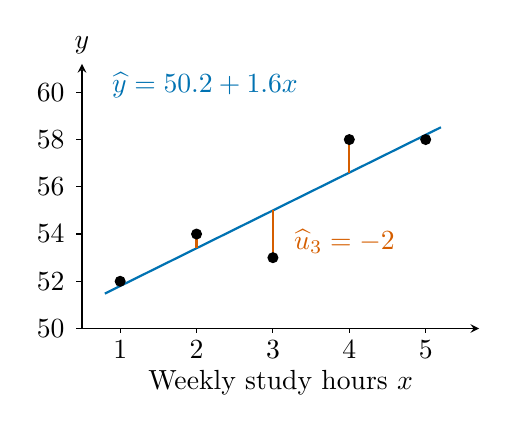
\begin{tikzpicture}[x=.97cm,y=.30cm,>=stealth]
\draw[->] (.5,0)--(5.7,0);
\draw[->] (.5,0)--(.5,11.2) node[above] {$y$};
\foreach \x in {1,2,3,4,5} {
  \draw (\x,0)--(\x,-.18);
  \node[below] at (\x,-.1) {$\x$};
}
\foreach \y/\lab in {0/50,2/52,4/54,6/56,8/58,10/60} {
  \draw (.5,\y)--(.42,\y);
  \node[left] at (.4,\y) {$\lab$};
}
\node[below] at (3.1,-1.35) {Weekly study hours $x$};
\draw[blue,thick] (.8,1.48)--(5.2,8.52);
\foreach \x/\y/\f in {1/2/1.8,2/4/3.4,3/3/5,4/8/6.6,5/8/8.2} {
  \draw[red,thick] (\x,\f)--(\x,\y);
  \fill[black] (\x,\y) circle[radius=2pt];
}
\node[blue,anchor=west,fill=white,inner sep=1pt] at (.85,10.3) {$\widehat y=50.2+1.6x$};
\node[red,anchor=west] at (3.15,3.7) {$\widehat u_3=-2$};
\end{tikzpicture}
\end{column}
\end{columns}
\vspace{.15cm}
Residuals use the estimated sample line. Population errors use the true population coefficients.
\end{frame}

\begin{frame}{Solution 3: Normal equations and squared errors (continued)}
\small
\answerpart{2}The normal equations are satisfied:
\begin{align*}
\sum_i\widehat u_i&=.2+.6-2+1.4-.2=0,\\
\sum_i x_i\widehat u_i&=1(.2)+2(.6)+3(-2)+4(1.4)+5(-.2)=0.
\end{align*}
The line passes through the sample means:
\[
\widehat y(\overline x)=\widehat\beta_0+\widehat\beta_1\overline x
=50.2+1.6(3)=55=\overline y.
\]
\answerpart{3}The OLS residual sum of squares is
\[
SSR=\sum_i\widehat u_i^2
=.2^2+.6^2+(-2)^2+1.4^2+(-.2)^2=\boxed{6.4}.
\]
\begin{center}
\begin{tabular}{l|c|r}
Prediction & Residuals & Sum of squared errors \\ \hline
Constant 55 & $-3,\,-1,\,-2,\,3,\,3$ & $32$ \\
Candidate $50+2x$ & $0,\,0,\,-3,\,0,\,-2$ & $13$ \\
OLS $50.2+1.6x$ & $.2,\,.6,\,-2,\,1.4,\,-.2$ & $6.4$
\end{tabular}
\end{center}
OLS has lower squared error than either alternative. These sample fitting identities do not establish causality.
\end{frame}
% SOLUTION 3 END
\fi

\begin{frame}{Problem 4: What does a 10-percentage-point increase predict?}
An estimated district regression relates the average test score $Y$ to the share $p$ of students receiving subsidized meals:
\[
\widehat y=850-150p.
\]
The observed shares range from $.20$ to $.80$. The standard deviation of district scores is 60 points.
\begin{enumerate}
\setlength{\itemsep}{8pt}
\item Predict scores at $p=.40$ and $p=.50$. Calculate the predicted change for this 10-percentage-point increase in the share.
\item Express the regressor as a percentage, $P=100p$. Rewrite the fitted line and state the slope's new units. Check that the same change still gives the same predicted score difference.
\item What does the line predict at $p=0$, and why does interpreting that value require extrapolation? Express the 15-point predicted decrease as a fraction of the outcome's standard deviation.
\end{enumerate}
\end{frame}
\note{All figures are hypothetical teaching data, not estimates from the California dataset in the lecture. Solution to Problem 4. At shares .4 and .5, predicted test scores are 790 and 775. Delta yhat=beta1hat Delta p=-150(.1)=-15 points. A one-unit change in p is 100 percentage points; a .1-unit change is 10 percentage points. With P=100p, the fitted line is 850-1.5P, whose slope is -1.5 score points per percentage point. Moving P from40 to50 again gives -1.5(10)=-15 points. The intercept predicts850 at p0, outside the observed range [.2,.8]; this is extrapolation rather than a prediction supported by observations near zero. The change is -15/60=-.25 standard deviations, a magnitude of one quarter of a standard deviation. The line describes an association and does not by itself identify a causal effect of subsidized meals.}

\ifshowsolutions
% SOLUTION 4 START
\begin{frame}{Solution 4: Shares, percentage points, and predicted scores}
\small
\answerpart{1}For a share $p$, the fitted score is $\widehat y(p)=850-150p$:
\[
\widehat y(.40)=850-150(.40)=790,
\qquad
\widehat y(.50)=850-150(.50)=775.
\]
\[
\Delta\widehat y=\widehat\beta_1\Delta p
=-150(.50-.40)=\boxed{-15\text{ points}}.
\]
A one-unit increase in the share means 100 percentage points. Here $\Delta p=.10$ means 10 percentage points.
\par\vspace{7pt}
\answerpart{2}Since $P=100p$, substitute $p=P/100$:
\[
\widehat y=850-150\left(\frac P{100}\right)=\boxed{850-1.5P}.
\]
The slope is now $-1.5$ test-score points per percentage point. In these units,
\[
\Delta\widehat y=(-1.5)(50-40)=\boxed{-15\text{ points}}.
\]
Changing the units changes the coefficient's numerical scale and preserves the predictions.
\end{frame}

\begin{frame}{Solution 4: The intercept and a standard-deviation benchmark (continued)}
\small
\answerpart{3}The line's value at zero share is
\[
\widehat y(0)=850-150(0)=\boxed{850\text{ points}}.
\]
But $p=0$ is outside the observed range $[.20,.80]$. Applying the fitted line there extrapolates beyond the available data; the intercept is not evidence about districts observed near zero share.
\par\vspace{10pt}
The predicted change relative to the outcome's standard deviation is
\[
\frac{\Delta\widehat y}{s_Y}
=\frac{-15}{60}=\boxed{-.25}.
\]
The 10-percentage-point increase in meal share is associated with a predicted score decrease of \textbf{one quarter of a standard deviation}.
\begin{block}{Interpretation}
The estimated line describes an association. A causal interpretation requires evidence about how meal shares and other determinants of scores are related.
\end{block}
\end{frame}
% SOLUTION 4 END
\fi

\begin{frame}{Problem 5: What does a tutoring indicator estimate?}
Let $D=1$ indicate tutoring participation and $D=0$ no tutoring. Six students have the following test scores:
\begin{center}
\begin{tabular}{c|rrr}
Group & \multicolumn{3}{c}{Scores $y_i$ (points)} \\ \hline
$D=0$ & 60 & 63 & 66 \\
$D=1$ & 67 & 70 & 73
\end{tabular}
\end{center}
Fit $\widehat y_i=\widehat\beta_0+\widehat\beta_1D_i$. No assignment mechanism is specified.
\begin{enumerate}
\setlength{\itemsep}{7pt}
\item Calculate each group's mean score, $\overline y_0$ and $\overline y_1$.
\item Split the OLS objective into sums for the two groups. Use the first-order conditions to explain why the intercept is $\overline y_0$ and the slope is $\overline y_1-\overline y_0$.
\item Calculate the fitted scores, residuals, and total $SSR$.
\item Does the slope identify a causal tutoring effect from these data alone? State a random-assignment design under which the difference could estimate an average causal effect.
\end{enumerate}
\end{frame}
\note{All scores are hypothetical teaching data. Solution to Problem 5. The group means are (60+63+66)/3=63 and (67+70+73)/3=70. The objective is sum over D0 of(yi-a) squared plus sum over D1 of(yi-a-b) squared. Its b first-order condition implies a+b=ybar1. Combining this with the a first-order condition implies a=ybar0, hence beta0hat63 and beta1hat7. Fitted values are63 for controls and70 for participants. Within each group the residuals are -3,0,3, so each group contributes18 to SSR and totalSSR36. With no assignment mechanism, the slope is a sample association. Individual random assignment, full take-up, no spillovers, and complete posttest follow-up permit interpreting the difference as an estimate of the average causal effect for the study population. Do not present a fitted group difference as causal merely because the binary-regressor OLS residuals average zero within each group.}

\ifshowsolutions
% SOLUTION 5 START
\begin{frame}{Solution 5: A binary slope is a difference in group means}
\small
\answerpart{1}For group $d$, $\overline y_d=n_d^{-1}\sum_{i:D_i=d}y_i$. Here,
\[
\overline y_0=\frac{60+63+66}{3}=63,
\qquad
\overline y_1=\frac{67+70+73}{3}=70.
\]
\answerpart{2}For candidate coefficients $(a,b)$, write
\[
Q(a,b)=\sum_{i:D_i=0}(y_i-a)^2
+\sum_{i:D_i=1}(y_i-a-b)^2.
\]
The first-order condition for $b$ gives
\[
\frac{\partial Q}{\partial b}=-2\sum_{i:D_i=1}(y_i-a-b)=0
\quad\Longrightarrow\quad a+b=\overline y_1.
\]
The first-order condition for $a$ then gives
\[
\frac{\partial Q}{\partial a}
=-2\sum_{i:D_i=0}(y_i-a)-2\underbrace{\sum_{i:D_i=1}(y_i-a-b)}_{=0}=0
\quad\Longrightarrow\quad a=\overline y_0.
\]
Thus
\[
\widehat\beta_0=\overline y_0=\boxed{63},
\qquad \widehat\beta_1=\overline y_1-\overline y_0=70-63=\boxed7.
\]
\end{frame}

\begin{frame}{Solution 5: Group predictions and a causal interpretation (continued)}
\small
\answerpart{3}Use $\widehat y_i=63+7D_i$ and $\widehat u_i=y_i-\widehat y_i$:
\begin{center}
\begin{tabular}{c|c|c|c}
Group & Observed scores & Fitted scores & Residuals \\ \hline
$D=0$ & $60,\ 63,\ 66$ & $63,\ 63,\ 63$ & $-3,\ 0,\ 3$ \\
$D=1$ & $67,\ 70,\ 73$ & $70,\ 70,\ 70$ & $-3,\ 0,\ 3$
\end{tabular}
\end{center}
\[
SSR=\sum_i\widehat u_i^2
=[(-3)^2+0^2+3^2]+[(-3)^2+0^2+3^2]
=18+18=\boxed{36\text{ points}^2}.
\]
\answerpart{4}With no assignment mechanism specified, the estimated slope describes a \textbf{7-point sample difference} between participants and nonparticipants.
\par\vspace{7pt}
If students were individually randomized to tutoring, with full take-up, no spillovers, and complete posttest follow-up, this difference could estimate the average causal effect for the study population.
\par\vspace{7pt}
Zero average residuals within groups are an OLS fitting property; they do not establish those design conditions.
\end{frame}
% SOLUTION 5 END
\fi

\section{Fit}

\begin{frame}{Problem 6: How much score variation does the line explain?}
Use the five observations and fitted values from Problems 2--3:
\begin{center}
\begin{tabular}{c|rrrrr}
$x_i$ & 1 & 2 & 3 & 4 & 5 \\
$y_i$ & 52 & 54 & 53 & 58 & 58 \\
$\widehat y_i$ & 51.8 & 53.4 & 55 & 56.6 & 58.2 \\
$\widehat u_i$ & .2 & .6 & $-2$ & 1.4 & $-.2$
\end{tabular}
\end{center}
The sample mean is $\overline y=55$.
\begin{enumerate}
\setlength{\itemsep}{8pt}
\item Compute the total sum of squares ($TSS$), explained sum of squares ($ESS$), and residual sum of squares ($SSR$). Verify $TSS=ESS+SSR$.
\item Calculate $R^2$ using both $ESS/TSS$ and $1-SSR/TSS$.
\item Calculate the sample variances of $Y$ and $\widehat Y$. Relate their ratio to $R^2$ and interpret the result.
\end{enumerate}
\end{frame}
\note{All numerical quantities are hypothetical teaching data. Solution to Problem 6. Deviations of Y from 55 are -3,-1,-2,3,3 and squared deviations are 9,1,4,9,9, summing to TSS32. Fitted deviations from 55 are -3.2,-1.6,0,1.6,3.2, with squares 10.24,2.56,0,2.56,10.24, summing to ESS25.6. Residual squares are .04,.36,4,1.96,.04, summing to SSR6.4. Hence 32=25.6+6.4. R squared equals 25.6/32=1-6.4/32=.8. Sample variances divide by n-1=4: sY squared=8 and fitted sample variance=6.4, ratio .8. The fitted line accounts for 80 percent of the observed variation in scores around their sample mean. This in-sample fit does not prove future predictive accuracy or causality. The decomposition and variance ratio here apply to OLS with an intercept.}

\ifshowsolutions
% SOLUTION 6 START
\begin{frame}{Solution 6: Decomposing the observed score variation}
\small
\answerpart{1}For OLS with an intercept, $\overline{\widehat y}=\overline y=55$. Define
\[
TSS=\sum_i(y_i-\overline y)^2,\quad
ESS=\sum_i(\widehat y_i-\overline y)^2,\quad
SSR=\sum_i\widehat u_i^2.
\]
\begin{center}
\begin{tabular}{c|rrr}
Student $i$ & $(y_i-55)^2$ & $(\widehat y_i-55)^2$ & $\widehat u_i^2$ \\
\hline
1 & 9 & 10.24 & .04 \\
2 & 1 & 2.56 & .36 \\
3 & 4 & 0 & 4 \\
4 & 9 & 2.56 & 1.96 \\
5 & 9 & 10.24 & .04 \\
\hline
Sum & $TSS=32$ & $ESS=25.6$ & $SSR=6.4$
\end{tabular}
\end{center}
Thus $TSS=ESS+SSR$: $32=25.6+6.4$.
\par\vspace{5pt}
\answerpart{2}Both expressions give
\[
R^2=\frac{ESS}{TSS}=\frac{25.6}{32}=\boxed{.8},
\qquad R^2=1-\frac{SSR}{TSS}=1-\frac{6.4}{32}=\boxed{.8}.
\]
\end{frame}

\begin{frame}{Solution 6: The variance ratio and its interpretation}
\small
\answerpart{3}Both sample variances use the same divisor $n-1$:
\[
s_Y^2=\frac{\sum_i(y_i-\overline y)^2}{n-1}
=\frac{32}{5-1}=8\text{ points}^2,
\]
\[
s_{\widehat Y}^2=\frac{\sum_i(\widehat y_i-\overline{\widehat y})^2}{n-1}
=\frac{25.6}{5-1}=6.4\text{ points}^2.
\]
Since the fitted values have mean $\overline y$,
\[
\frac{s_{\widehat Y}^2}{s_Y^2}
=\frac{ESS/(n-1)}{TSS/(n-1)}
=\frac{ESS}{TSS}=\frac{6.4}{8}=\boxed{.8=R^2}.
\]
The fitted line accounts for 80\% of the observed variation in scores around their sample mean. The remaining 20\% is in the residuals.

\par\vspace{5pt}
This describes fit in these five observations. It does not by itself establish accuracy on future data or a causal effect of study hours.
\end{frame}
% SOLUTION 6 END
\fi

\begin{frame}{Problem 7: How large are the residuals around the line?}
Use Problems 2--3: $n=5$, $\widehat y=50.2+1.6x$, $SSR=6.4$, and $TSS=32$.
\begin{enumerate}
\setlength{\itemsep}{12pt}
\item Calculate $SER^2$ and $SER$. Compare $SER$ with the sample standard deviation $s_Y$ of scores.
\item Calculate the in-sample root mean squared error, $RMSE$. Explain why its denominator differs from that of $SER$.
\item Predict the score at $x=3.5$ study hours and calculate $\widehat y\pm SER$. Is this automatically a 95\% prediction interval for a new student's score? Explain.
\end{enumerate}
\end{frame}
\note{All numerical quantities are hypothetical teaching data. Solution to Problem 7. SER squared=SSR/(n-2)=6.4/3=32/15=2.13333 points squared and SER=sqrt(32/15)=1.46059 points. Sample score SD=sqrt(TSS/(n-1))=sqrt(32/4)=sqrt8=2.82843 points. SER describes residual dispersion around the fitted line, whereas sY describes score dispersion around the sample mean. In-sample RMSE=sqrt(SSR/n)=sqrt(6.4/5)=sqrt1.28=1.13137 points. SER uses three residual degrees of freedom after estimating two coefficients; RMSE uses five observations to average squared sample errors. Neither is a coefficient standard error. Predicted score at 3.5 hours=50.2+1.6(3.5)=55.8; plus/minus SER is [54.3394,57.2606]. This is a descriptive one-residual-SD band, not a guaranteed 95 percent prediction interval. A formal prediction interval needs appropriate error-distribution assumptions, a critical value, and uncertainty in both the future error and estimated coefficients.}

\ifshowsolutions
% SOLUTION 7 START
\begin{frame}{Solution 7: SER, RMSE, and their denominators}
\small
\answerpart{1}Two fitted coefficients leave $n-2$ residual degrees of freedom:
\[
SER^2=\frac{SSR}{n-2}=\frac{6.4}{5-2}=\frac{32}{15}\approx2.1333\text{ points}^2,
\]
\[
SER=\sqrt{SER^2}=\sqrt{\frac{32}{15}}\approx\boxed{1.4606\text{ points}}.
\]
For comparison,
\[
s_Y=\sqrt{\frac{TSS}{n-1}}=\sqrt{\frac{32}{4}}=\sqrt8\approx2.8284\text{ points}.
\]
$SER$ measures residual spread around the line; $s_Y$ measures spread around the sample mean.
\par\vspace{5pt}
\answerpart{2}The in-sample average squared error divides by all $n$ observations:
\[
RMSE=\sqrt{\frac1n\sum_i\widehat u_i^2}
=\sqrt{\frac{SSR}{n}}=\sqrt{\frac{6.4}{5}}=\sqrt{1.28}\approx\boxed{1.1314\text{ points}}.
\]
Thus $SER>RMSE$: their squared numerators agree, but their divisors are 3 and 5. Neither quantity is the standard error of a regression coefficient.
\end{frame}

\begin{frame}{Solution 7: Predicting at three and a half study hours}
\small
\answerpart{3}Insert $x=3.5$ into the fitted line:
\[
\widehat y(x)=\widehat\beta_0+\widehat\beta_1x,
\qquad
\widehat y(3.5)=50.2+1.6(3.5)=\boxed{55.8\text{ points}}.
\]
A band extending one $SER$ on either side is
\[
\widehat y(3.5)\pm SER
=55.8\pm\sqrt{32/15}
\approx\boxed{[54.339,\ 57.261]}\text{ points}.
\]
This is a descriptive one-residual-standard-deviation band. It does not automatically have 95\% coverage for a new student's score.

\par\vspace{8pt}
A formal prediction interval needs a suitable error-distribution model and critical value. It must also account for uncertainty in the new student's error and the estimated regression coefficients.
\end{frame}
% SOLUTION 7 END
\fi

\section{Assumptions}

\begin{frame}{Problem 8: Can the best line miss the conditional mean?}
A finite population has $X\in\{-1,0,1\}$, each with probability $1/3$, and $Y=X^2$. The population best linear predictor minimizes
\[
Q(a,b)=\E[(Y-a-bX)^2].
\]
Denote its coefficients by $\beta_0^*$ and $\beta_1^*$.
\begin{enumerate}
\setlength{\itemsep}{9pt}
\item Compute $\E(X)$, $\E(Y)$, $\Var(X)$, and $\Cov(X,Y)$. Use the population first-order conditions to find $\beta_0^*$ and $\beta_1^*$.
\item Compare the best linear predictor $\beta_0^*+\beta_1^*x$ with the true conditional mean $\E(Y\mid X=x)$ at all three values of $x$.
\item Define the population projection error $V=Y-\beta_0^*-\beta_1^*X$. Verify $\E(V)=\E(XV)=0$. Is $\E(V\mid X)=0$ also true?
\end{enumerate}
\end{frame}
\note{This is a hypothetical finite teaching population, not a causal model. Solution to Problem 8. E(X)=0, E(Y)=2/3, E(X squared)=2/3, Var(X)=2/3, E(XY)=E(X cubed)=0 and Cov(X,Y)=0. The population first-order conditions E(Y-a-bX)=0 and E[X(Y-a-bX)]=0 imply a=E(Y)-bE(X), b=Cov(X,Y)/Var(X)=0. Therefore beta0 star=2/3 and beta1 star=0. The best line is constant 2/3, whereas the conditional mean is x squared: 1,0,1. Projection errors at X=-1,0,1 are 1/3,-2/3,1/3. Their mean is zero, and E(XV)=[-1/3+0+1/3]/3=0. Yet E(V|X=x)=x squared-2/3 is never zero on the support. Thus zero covariance is weaker than zero conditional mean. A nonzero conditional mean does not necessarily imply nonzero covariance. The stars denote population projection coefficients, not sample estimates.}

\ifshowsolutions
% SOLUTION 8 START
\begin{frame}{Solution 8: Finding the population best line}
\small
\answerpart{1}Using equal probabilities,
\[
\E(X)=\frac{-1+0+1}{3}=0,\qquad
\E(Y)=\E(X^2)=\frac{1+0+1}{3}=\frac23,
\]
\[
\Var(X)=\E(X^2)-[\E(X)]^2=\frac23,
\qquad
\Cov(X,Y)=\E(XY)-\E(X)\E(Y)=\E(X^3)=0.
\]
The population first-order conditions for $Q(a,b)$ are
\[
\frac{\partial Q}{\partial a}=-2\E(Y-a-bX)=0,
\qquad
\frac{\partial Q}{\partial b}=-2\E[X(Y-a-bX)]=0.
\]
The first gives $a=\E(Y)-b\E(X)$. Substituting into the second gives
\[
\Cov(X,Y)-b\Var(X)=0
\quad\Longrightarrow\quad
\beta_1^*=\frac{\Cov(X,Y)}{\Var(X)}=0,
\]
\[
\beta_0^*=\E(Y)-\beta_1^*\E(X)=\boxed{\frac23}.
\]
These are population projection coefficients, rather than sample estimates.
\end{frame}

\begin{frame}{Solution 8: Orthogonality and conditional means}
\small
\answerpart{2}Since $Y=X^2$ deterministically, $\E(Y\mid X=x)=x^2$.
\begin{center}
\begin{tabular}{c|ccc}
$x$ & $-1$ & $0$ & $1$ \\
\hline
True conditional mean $x^2$ & 1 & 0 & 1 \\
Best linear predictor $\beta_0^*+\beta_1^*x$ & $2/3$ & $2/3$ & $2/3$ \\
Projection error $V$ & $1/3$ & $-2/3$ & $1/3$
\end{tabular}
\end{center}
\answerpart{3}The projection error is $V=Y-2/3$. Therefore
\[
\E(V)=\frac{1/3-2/3+1/3}{3}=0,
\qquad
\E(XV)=\frac{-1/3+0+1/3}{3}=0.
\]
However,
\[
\E(V\mid X=x)=x^2-\frac23\ne0
\quad\text{for every }x\in\{-1,0,1\}.
\]
The error is uncorrelated with $X$, but its conditional mean is nonzero. Zero covariance is weaker than zero conditional mean; this example concerns prediction, not a causal effect.
\end{frame}
% SOLUTION 8 END
\fi

\begin{frame}{Problem 9: Can disadvantage reverse the observed tutoring gap?}
Suppose the structural model for test scores is
\[
Y=80+5D-10Z+V,
\]
where $D$ indicates tutoring participation and $Z$ measures disadvantage. Assume finite second moments. In this model, changing $D$ from 0 to 1 while holding $Z$ and $V$ fixed raises the score by 5 points. Assume
\[
\E(V\mid D)=0,\quad
\E(Z\mid D=0)=1,\quad \E(Z\mid D=1)=2,\quad
\Pr(D=1)=.5.
\]
\begin{enumerate}
\setlength{\itemsep}{8pt}
\item Calculate $\E(Y\mid D=0)$, $\E(Y\mid D=1)$, and the observed mean gap.
\item If $Z$ is omitted, define the structural error $U=-10Z+V$. Compute $\E(U\mid D=0)$ and $\E(U\mid D=1)$. Does zero conditional mean hold?
\item Find $\Var(D)$ and $\Cov(D,U)$. Derive the population regression slope of $Y$ on $D$, and explain why it differs from the structural effect.
\end{enumerate}
\end{frame}
\note{All numerical quantities and the structural model are hypothetical teaching examples. Solution to Problem 9. Conditional means are 80+5d-10E(Z|D=d)+E(V|D=d), giving 70 for D0 and 65 for D1. Observed gap=-5. The omitted structural error U=-10Z+V has conditional means -10 and -20, so E(U|D)=0 fails and the conditional mean differs by group. E(D)=.5 and Var(D)=.5(1-.5)=.25. E(U)=.5(-10)+.5(-20)=-15. E(DU)=.5(-20)=-10; Cov(D,U)=-10-.5(-15)=-2.5. The population slope equals Cov(D,Y)/Var(D)=5+Cov(D,U)/Var(D)=5-10=-5. The intercept is 70. By construction the structural ceteris paribus effect is positive 5, but greater disadvantage among participants reverses the observational association. U is the structural error from retaining coefficients 80 and 5 while omitting Z. It is not the error from the population linear projection: that error is Y-70+5D and has zero group-conditional mean for this binary regressor. Sample OLS residual orthogonality is a normal-equation property and does not establish the structural error condition or causality.}

\ifshowsolutions
% SOLUTION 9 START
\begin{frame}{Solution 9: Group means and the omitted structural error}
\small
\answerpart{1}Take conditional expectations of the structural equation:
\[
\E(Y\mid D=d)=80+5d-10\E(Z\mid D=d)+\E(V\mid D=d).
\]
Hence
\[
\E(Y\mid D=0)=80-10(1)=70,
\qquad
\E(Y\mid D=1)=80+5-10(2)=65.
\]
The observed mean gap is $65-70=\boxed{-5\text{ points}}$.
\par\vspace{8pt}
\answerpart{2}With $U=-10Z+V$,
\[
\E(U\mid D=d)=-10\E(Z\mid D=d)+\E(V\mid D=d),
\]
\[
\E(U\mid D=0)=-10,
\qquad
\E(U\mid D=1)=-20.
\]
The structural error has nonzero conditional means that differ across tutoring groups. The zero-conditional-mean assumption fails.
\end{frame}

\begin{frame}{Solution 9: The population slope and the structural effect}
\small
\answerpart{3}For binary $D$ with $p=\Pr(D=1)$, $\Var(D)=p(1-p)=.25$. Also,
\[
\E(U)=\sum_{d=0}^1\E(U\mid D=d)\Pr(D=d)
=.5(-10)+.5(-20)=-15,
\]
\[
\E(DU)=\Pr(D=1)\E(U\mid D=1)=.5(-20)=-10,
\]
\[
\Cov(D,U)=\E(DU)-\E(D)\E(U)=-10-(.5)(-15)=-2.5.
\]
From $Y=80+5D+U$, the population projection slope is
\[
\beta_1^*=\frac{\Cov(D,Y)}{\Var(D)}
=5+\frac{\Cov(D,U)}{\Var(D)}
=5+\frac{-2.5}{.25}=\boxed{-5}.
\]
The structural effect is $+5$ points, but greater disadvantage among participants creates a negative observational gap.

\par\vspace{5pt}
The omitted structural error $U$ differs from a projection error or a sample OLS residual. Orthogonality of OLS residuals does not establish structural exogeneity or causality.
\end{frame}
% SOLUTION 9 END
\fi

\begin{frame}{Problem 10: One unusual score and repeated students}
Return to Problem 2, with $x=(1,2,3,4,5)$ and $y=(52,54,53,58,58)$. Replace only the last score, $y_5=58$, by 90. Originally, $\overline x=3$, $S_{XX}=10$, and $\widehat\beta_1=1.6$.
\begin{enumerate}
\setlength{\itemsep}{10pt}
\item Recalculate $\overline y$, $S_{XY}$, the OLS slope, and the intercept using the changed data.
\item Derive the change in the slope when only one $y_j$ changes. Apply it here with $\Delta y_5=32$. What should we investigate before deciding how to handle this observation?
\item Compare two designs: 100 independent draws from the same student population, versus 20 weekly observations for each of five students. Is i.i.d. sampling justified equally in both? If hours and scores are bounded, what does that imply about fourth moments, independence, and influential observations?
\end{enumerate}
\end{frame}
\note{All numerical quantities and sampling designs are hypothetical teaching examples. Solution to Problem 10. New scores sum to 307 and have mean61.4. Centered cross-products with unchanged xbar3 are 18.8,7.4,0,-3.4,57.2, sum80. With SXX10, new slope8 and intercept61.4-8(3)=37.4. Since sum(xi-xbar)=0, SXY can be written sum(xi-xbar)yi. If X stays fixed and only yj changes, delta slope=(xj-xbar)delta yj/SXX. Here 2(32)/10=6.4 and 1.6+6.4=8. Investigate recording/coding error, units, context, and whether 90 is a valid extreme outcome; do not delete a valid observation just because it changes the fit. Independent draws from the same student population support i.i.d. at the student level. Repeated weekly observations may share student-specific factors and temporal dependence, so treating 100 records from five students as 100 independent draws is unjustified without further assumptions. Bounded X,Y have finite fourth moments, but boundedness does not imply independence and does not prevent an observation from exerting substantial influence in a small sample.}

\ifshowsolutions
% SOLUTION 10 START
\begin{frame}{Solution 10: Re-estimating after changing one score}
\small
\answerpart{1}The regressor values are unchanged, so $\overline x=3$ and $S_{XX}=10$. With the new score,
\[
\overline y_{\mathrm{new}}=\frac1n\sum_i y_{i,\mathrm{new}}
=\frac{52+54+53+58+90}{5}=\frac{307}{5}=61.4.
\]
\[
\begin{aligned}
S_{XY,\mathrm{new}}
&=\sum_i(x_i-\overline x)(y_{i,\mathrm{new}}-\overline y_{\mathrm{new}})\\
&=18.8+7.4+0-3.4+57.2=80.
\end{aligned}
\]
The new coefficients are
\[
\widehat\beta_{1,\mathrm{new}}=\frac{S_{XY,\mathrm{new}}}{S_{XX}}=\frac{80}{10}=\boxed{8},
\]
\[
\widehat\beta_{0,\mathrm{new}}=\overline y_{\mathrm{new}}-\widehat\beta_{1,\mathrm{new}}\overline x
=61.4-8(3)=\boxed{37.4}.
\]
Changing one score moves the fitted line from $50.2+1.6x$ to $37.4+8x$.
\end{frame}

\begin{frame}{Solution 10: Influence and the unit of sampling (continued)}
\small
\answerpart{2}Since $\sum_i(x_i-\overline x)=0$, write
\[
\widehat\beta_1=\frac{\sum_i(x_i-\overline x)y_i}{S_{XX}}.
\]
With all $x_i$ fixed and only $y_j$ changed,
\[
\Delta\widehat\beta_1=\frac{(x_j-\overline x)\Delta y_j}{S_{XX}}
=\frac{(5-3)(90-58)}{10}=6.4,
\qquad 1.6+6.4=8.
\]
Check recording, coding, units, and context. A valid extreme score should not be deleted automatically because it changes the line.
\par\vspace{6pt}
\answerpart{3}Independent draws from the same student population support the i.i.d. assumption at the student level. Repeated observations of five students may share individual factors and dependence over time; 100 records need not be 100 independent observations.

\par\vspace{6pt}
Bounded hours and scores have finite fourth moments. Boundedness does not guarantee independence or prevent a realized observation from strongly influencing a small-sample regression.
\end{frame}
% SOLUTION 10 END
\fi

\section{Precision}

\begin{frame}{Problem 11: Are both OLS coefficients unbiased?}
For the full regressor sample $\mathbf X=(1,2,3)$, outcomes satisfy
\[
Y_i=10+2X_i+U_i.
\]
Conditional on the full $\mathbf X$, the errors are independent and each equals $-1$ or $1$ with probability $1/2$.
\begin{enumerate}
\setlength{\itemsep}{7pt}
\item Show that $\E[X_iU_i\mid\mathbf X]=X_i\E[U_i\mid\mathbf X]=0$. Why can $X_i$ be taken outside this expectation?
\item With $\overline X=2$ and $S_{XX}=\sum_i(X_i-\overline X)^2=2$, express each OLS coefficient as its true value plus a weighted sum of errors. Find their conditional means. How does iterated expectations extend the result to random regressors?
\item List the possible values of $\widehat\beta_1$, their probabilities, and their mean.
\end{enumerate}
\end{frame}
\note{All numerical values are invented for teaching. Solution to Problem 11. Conditioning is on the full vector, not merely on each observation's Xi. Xi and all OLS weights are known under that conditioning. Each error has conditional expectation zero. Slope error equals (U3-U1)/2. Intercept error equals Ubar minus2 times slope error, hence (4U1+U2-2U3)/3. Their conditional expectations are2 and10. Under random regressors, maintain zero conditional means given the full vector, Sxx positive almost surely, and finite expectations of the estimators, and apply iterated expectations. No large-sample approximation is required. Independence of U1 and U3 gives slope1 with probability1/4,2 with probability1/2,3 with probability1/4; weighted mean2. U2 has no influence on the slope in this centered design.}

\ifshowsolutions
% SOLUTION 11 START
\begin{frame}{Solution 11: Fixed conditional weights}
\small
\answerpart{1}Given $\mathbf X$, each $X_i$ is a known constant. Since
\[
\E[U_i\mid\mathbf X]=(-1)\frac12+(1)\frac12=0,
\qquad
\E[X_iU_i\mid\mathbf X]=X_i\E[U_i\mid\mathbf X]=\boxed0.
\]
\answerpart{2}The OLS slope error is a weighted sum:
\begin{align*}
\widehat\beta_1-\beta_1
&=\frac{\sum_i(X_i-\overline X)U_i}{S_{XX}}
=\frac{-U_1+0U_2+U_3}{2},\\
\widehat\beta_1&=\boxed{2+\frac{U_3-U_1}{2}}.
\end{align*}
The intercept uses $\overline Y=\beta_0+\beta_1\overline X+\overline U$:
\begin{align*}
\widehat\beta_0-\beta_0
&=\overline U-\overline X(\widehat\beta_1-\beta_1)\\
&=\frac{U_1+U_2+U_3}{3}-2\frac{U_3-U_1}{2}
=\frac{4U_1+U_2-2U_3}{3}.
\end{align*}
Thus $\boxed{\widehat\beta_0=10+(4U_1+U_2-2U_3)/3}$.
\end{frame}

\begin{frame}{Solution 11: Unbiasedness and a slope distribution (continued)}
\small
\answerpart{2}Taking conditional expectations of the error expressions gives
\[
\E[\widehat\beta_1\mid\mathbf X]
=2+\frac{\E[U_3\mid\mathbf X]-\E[U_1\mid\mathbf X]}{2}=\boxed2,
\]
\[
\E[\widehat\beta_0\mid\mathbf X]
=10+\frac{4\E[U_1\mid\mathbf X]+\E[U_2\mid\mathbf X]-2\E[U_3\mid\mathbf X]}3
=\boxed{10}.
\]
If $\mathbf X$ is random, the same argument applies whenever $S_{XX}>0$ and $\E[U_i\mid\mathbf X]=0$. With finite coefficient expectations,
\[
\E[\widehat\beta_j]=\E\!\left[\E[\widehat\beta_j\mid\mathbf X]\right]
=\beta_j,\qquad j=0,1.
\]
\answerpart{3}Independence makes the four $(U_1,U_3)$ pairs equally likely:
\begin{center}
\begin{tabular}{c|ccc}
$\widehat\beta_1$ & 1 & 2 & 3\\ \hline
Probability & $1/4$ & $1/2$ & $1/4$
\end{tabular}
\end{center}
\[
\E[\widehat\beta_1\mid\mathbf X]=\sum_b b\Pr(\widehat\beta_1=b\mid\mathbf X)
=1\!\left(\frac14\right)+2\!\left(\frac12\right)+3\!\left(\frac14\right)=2.
\]
Unbiasedness here is a finite-sample result; no large-$n$ approximation is used.
\end{frame}
% SOLUTION 11 END
\fi

\begin{frame}{Problem 12: How uncertain are the slope and intercept?}
Use the design from Problem 2: $X=(1,2,3,4,5)$, $n=5$, $\overline X=3$, and $S_{XX}=10$. In the population model $Y_i=\beta_0+\beta_1X_i+U_i$, assume, conditional on the full $\mathbf X$, mean-zero, uncorrelated errors with common variance $\sigma_U^2=4$.
\begin{enumerate}
\setlength{\itemsep}{8pt}
\item Use the fixed slope weights to derive $\Var(\widehat\beta_1\mid\mathbf X)$, then calculate its theoretical standard deviation.
\item Write the intercept error using weights $a_i=1/n-\overline X(X_i-\overline X)/S_{XX}$. Derive its conditional variance and calculate its theoretical standard deviation.
\item Now treat $\sigma_U^2$ as unknown. Use Problem 7's $SSR=6.4$ to estimate the standard errors of both coefficients. Distinguish these from the theoretical standard deviations above.
\end{enumerate}
\end{frame}
\note{All quantities are invented for teaching. Solution to Problem 12. With fixed Xi and conditionally uncorrelated errors, slope variance is sigmaU squared times sum of slope weights squared=sigmaU squared/Sxx=4/10=.4 and SD=sqrt(.4)=.6324555. Intercept variance is sigmaU squared times sum ai squared, with sum ai squared=1/n+xbar squared/Sxx=1/5+9/10=1.1. Intercept variance4.4, SD2.0976177. Estimated error variance SER squared=SSR/(n-2)=6.4/3=32/15. Estimated slope SE=sqrt((32/15)/10)=.4618802; intercept SE=sqrt((32/15)*(1/5+9/10))=1.5318834. These estimates can differ from the true SDs in one sample. With n5, do not invoke the large-sample normal approximation for tests or intervals.}

\ifshowsolutions
% SOLUTION 12 START
\begin{frame}{Solution 12: The slope's conditional variance}
\small
\answerpart{1}Let $d_i=X_i-\overline X$ and $w_i=d_i/S_{XX}$. Then
\[
\widehat\beta_1-\beta_1=\sum_iw_iU_i,
\qquad (w_1,w_2,w_3,w_4,w_5)=\frac1{10}(-2,-1,0,1,2).
\]
The weights are fixed given $\mathbf X$. Conditional cross covariances vanish:
\begin{align*}
\Var(\widehat\beta_1\mid\mathbf X)
&=\sum_iw_i^2\Var(U_i\mid\mathbf X)
=\sigma_U^2\sum_i\frac{d_i^2}{S_{XX}^2}\\
&=\frac{\sigma_U^2S_{XX}}{S_{XX}^2}
=\frac{\sigma_U^2}{S_{XX}}=\frac4{10}=\boxed{.4}.
\end{align*}
Its theoretical standard deviation is the square root:
\[
\operatorname{SD}(\widehat\beta_1\mid\mathbf X)
=\sqrt{\Var(\widehat\beta_1\mid\mathbf X)}
=\sqrt{.4}\approx\boxed{.63246}.
\]
These calculations use the population error variance $\sigma_U^2=4$.
\end{frame}

\begin{frame}{Solution 12: The intercept's conditional variance (continued)}
\small
\answerpart{2}The intercept error can also be written as a fixed weighted sum:
\[
\widehat\beta_0-\beta_0
=\overline U-\overline X\frac{\sum_id_iU_i}{S_{XX}}
=\sum_i a_iU_i,
\qquad a_i=\frac1n-\frac{\overline Xd_i}{S_{XX}}.
\]
Using $\sum_i d_i=0$ and $\sum_i d_i^2=S_{XX}$,
\begin{align*}
\sum_i a_i^2
&=\frac1n-\frac{2\overline X}{nS_{XX}}\underbrace{\sum_id_i}_{0}
+\frac{\overline X^2}{S_{XX}^2}\underbrace{\sum_id_i^2}_{S_{XX}}\\
&=\frac1n+\frac{\overline X^2}{S_{XX}}.
\end{align*}
Thus conditional uncorrelatedness gives
\[
\Var(\widehat\beta_0\mid\mathbf X)
=\sigma_U^2\sum_i a_i^2
=4\left(\frac15+\frac9{10}\right)=\boxed{4.4},
\]
\[
\operatorname{SD}(\widehat\beta_0\mid\mathbf X)=\sqrt{4.4}\approx\boxed{2.09762}.
\]
\end{frame}

\begin{frame}{Solution 12: Estimating both standard errors (continued)}
\small
\answerpart{3}Replace the unknown population error variance by
\[
\widehat\sigma_U^2=SER^2=\frac{SSR}{n-2}
=\frac{6.4}{5-2}=\frac{32}{15}.
\]
Take the square root of each estimated coefficient variance:
\begin{align*}
SE(\widehat\beta_1)
&=\sqrt{\frac{SER^2}{S_{XX}}}
=\sqrt{\frac{32/15}{10}}
\approx\boxed{.46188},\\[5pt]
SE(\widehat\beta_0)
&=\sqrt{SER^2\left(\frac1n+\frac{\overline X^2}{S_{XX}}\right)}\\
&=\sqrt{\frac{32}{15}\left(\frac15+\frac9{10}\right)}
\approx\boxed{1.53188}.
\end{align*}
The theoretical SDs use the true $\sigma_U^2=4$; the estimated SEs use the sample's $SER^2=32/15$. The latter vary across samples and need not equal the theoretical SDs in a particular sample.
\par\vspace{7pt}
With only five observations, these variance calculations do not by themselves justify large-sample normal tests or intervals.
\end{frame}
% SOLUTION 12 END
\fi

\begin{frame}{Problem 13: What makes a slope estimate precise?}
Three fixed designs satisfy the mean-zero, conditionally uncorrelated error assumptions, with $\sigma_U=4$:
\begin{center}
\begin{tabular}{c|rrr}
Design & $n$ & $\overline X$ & $S_{XX}$\\ \hline
$A$ & 100 & 0 & 100\\
$B$ & 100 & 0 & 400\\
$C$ & 400 & 0 & 400
\end{tabular}
\end{center}
\begin{enumerate}
\setlength{\itemsep}{6pt}
\item Calculate the theoretical conditional SDs of both OLS coefficients in each design. Explain the roles of regressor variation and sample size.
\item How do all these SDs change if $\sigma_U$ doubles to 8?
\item A fourth design has $n=100$, $\overline X=10$, and $S_{XX}=100$. Calculate both SDs. Then recenter with $Z=X-10$ and calculate the new intercept's SD. What changes in the meaning of the intercept?
\end{enumerate}
\end{frame}
\note{All designs are invented for teaching. Solution to Problem 13. Slope SD=sigmaU/sqrt(Sxx); intercept SD=sigmaU sqrt(1/n+xbar squared/Sxx). A slope.4/intercept.4;B .2/.4;C .2/.2. A toB increases X spread with same n, improving slope precision;B toC keeps total Sxx fixed, so slope precision stays same despite more observations. At xbar0 the intercept is the sample mean location and depends on n. Doubling sigmaU doubles all coefficient SDs, quadrupling variances. Fourth design slope.4, intercept sqrt(16.16)=4.0199502. Z centering leaves Szz100 and slope unchanged, but moves intercept target from conditional mean at old X0 to old X10. New intercept SD4/sqrt100=.4. The fitted value and its precision at every given old X are unchanged by reparameterization; precision is higher at the sample mean than at distant zero.}

\ifshowsolutions
% SOLUTION 13 START
\begin{frame}{Solution 13: Regressor spread, sample size, and noise}
\small
\answerpart{1}Take square roots of the conditional coefficient variances:
\[
\operatorname{SD}(\widehat\beta_1\mid\mathbf X)
=\sqrt{\frac{\sigma_U^2}{S_{XX}}}
=\frac{\sigma_U}{\sqrt{S_{XX}}},\qquad
\operatorname{SD}(\widehat\beta_0\mid\mathbf X)
=\sigma_U\sqrt{\frac1n+\frac{\overline X^2}{S_{XX}}}.
\]
\begin{center}
\begin{tabular}{c|cc}
Design & Slope SD & Intercept SD\\ \hline
$A$ & $4/\sqrt{100}=\boxed{.4}$ & $4\sqrt{1/100}=\boxed{.4}$\\[6pt]
$B$ & $4/\sqrt{400}=\boxed{.2}$ & $4\sqrt{1/100}=\boxed{.4}$\\[6pt]
$C$ & $4/\sqrt{400}=\boxed{.2}$ & $4\sqrt{1/400}=\boxed{.2}$
\end{tabular}
\end{center}
From A to B, more variation in $X$ halves the slope SD. From B to C, $S_{XX}$ stays fixed, so the slope SD stays fixed despite the larger $n$. With $\overline X=0$, the intercept SD falls as $1/\sqrt n$.
\par\vspace{6pt}
\answerpart{2}Both SD formulas are proportional to $\sigma_U$. Doubling $\sigma_U$ to 8 doubles every SD; it multiplies every variance by four.
\end{frame}

\begin{frame}{Solution 13: Where is the intercept measured? (continued)}
\small
\answerpart{3}For $n=100$, $\overline X=10$, and $S_{XX}=100$,
\begin{align*}
\operatorname{SD}(\widehat\beta_1\mid\mathbf X)
&=\sqrt{\frac{16}{100}}=\boxed{.4},\\[4pt]
\operatorname{SD}(\widehat\beta_0\mid\mathbf X)
&=\sqrt{16\left(\frac1{100}+\frac{10^2}{100}\right)}
=\sqrt{16.16}\approx\boxed{4.020}.
\end{align*}
If $Z=X-10$, then $\overline Z=0$ and $S_{ZZ}=S_{XX}=100$. Write
\[
Y=\gamma_0+\beta_1Z+U,
\qquad \gamma_0=\beta_0+10\beta_1.
\]
The new intercept estimates the line at old $X=10$, rather than old $X=0$:
\[
\operatorname{SD}(\widehat\gamma_0\mid\mathbf X)
=\sqrt{16\left(\frac1{100}+\frac{0^2}{100}\right)}=\boxed{.4}.
\]
The slope and fitted line are unchanged. Recentring changes the intercept's target; it does not improve the precision of the fitted line at any given $X$.
\end{frame}
% SOLUTION 13 END
\fi

\begin{frame}{Problem 14: Is the intercept or slope different from zero?}
Regress test-score gains $Y$ (points) on weekly tutoring hours $X$. A large i.i.d. sample gives
\[
n=102,\quad\overline X=10,\quad S_{XX}=400,\quad SSR=400,
\qquad\widehat\beta_0=1.5,\quad\widehat\beta_1=.3.
\]
Assume zero conditional-mean errors, conditionally uncorrelated errors, finite fourth moments, and a valid large-sample normal approximation.
\begin{enumerate}
\setlength{\itemsep}{5pt}
\item Calculate $SER$ and the estimated SEs of both coefficients.
\item State a two-sided zero-null test for each coefficient and compute each observed test statistic.
\item Find both approximate p-values and give the 5\% decisions. Use $\Phi(3)=.99865$ and $\Phi(1.4714)\approx.9294$.
\item Construct a 95\% confidence interval for each coefficient and check whether it contains zero. Are these two separate tests a joint test of both coefficients?
\end{enumerate}
\end{frame}
\note{All regression summaries are invented for teaching. Solution to Problem 14. SER=sqrt(SSR/(n-2))=sqrt400/100=2. Slope SE=SER/sqrtSxx=.1;intercept SE=SER sqrt(1/n+xbar squared/Sxx)=2sqrt(1/102+100/400)=1.019419289. Nulls beta1=0 vsneq0 and beta0=0 vsneq0. t1=.3/.1=3;t0=1.5/1.019419289=1.471425955. Approximate normal pvalues .0027 and .1412;reject slope zero at5 percent,do not reject intercept zero. Slope95CI .3 plusminus1.96(.1)=[.104,.496]. Intercept95CI1.5 plusminus1.96(1.019419289)=[-.498061806,3.498061806],rounded[-.498,3.498]. Zero excluded only by slope CI. These are separate marginal tests and intervals, not a joint test or simultaneous95percent confidence region. Use normal approximation as lecture, not an exact t distribution. The intercept is the line's population mean gain at zero tutoring hours; slope is points per additional weekly tutoring hour. No assignment mechanism is specified, so statistical significance alone does not establish a causal effect.}

\ifshowsolutions
% SOLUTION 14 START
\begin{frame}{Solution 14: Estimate the error variance and both SEs}
\small
\answerpart{1}With an intercept and one slope, the error variance estimate uses $n-2$:
\[
SER^2=\frac{SSR}{n-2}=\frac{400}{102-2}=4,
\qquad SER=\sqrt{\frac{SSR}{n-2}}=\sqrt4=\boxed2\text{ points}.
\]
Each coefficient SE is the square root of its estimated variance:
\begin{align*}
SE(\widehat\beta_1)
&=\sqrt{\frac{SER^2}{S_{XX}}}
=\sqrt{\frac4{400}}=\sqrt{.01}=\boxed{.1},\\[6pt]
SE(\widehat\beta_0)
&=\sqrt{SER^2\left(\frac1n+\frac{\overline X^2}{S_{XX}}\right)}\\
&=\sqrt{4\left(\frac1{102}+\frac{100}{400}\right)}
\approx\boxed{1.01942}.
\end{align*}
The slope SE is measured in points per weekly tutoring hour; the intercept SE is measured in points.
\end{frame}

\begin{frame}{Solution 14: Two separate zero-null tests (continued)}
\small
\answerpart{2}For each coefficient $j$, the zero-null statistic is
\[
t_j^{\mathrm{obs}}=\frac{\widehat\beta_j-0}{SE(\widehat\beta_j)}.
\]
\begin{center}
\begin{tabular}{c|c|c}
Coefficient & Hypotheses & Observed statistic\\ \hline
Slope & $H_0:\beta_1=0$ vs. $H_1:\beta_1\ne0$ & $.3/.1=\boxed3$\\[7pt]
Intercept & $H_0:\beta_0=0$ vs. $H_1:\beta_0\ne0$ & $1.5/1.01942\approx\boxed{1.4714}$
\end{tabular}
\end{center}
\answerpart{3}Under its null, use the large-sample normal approximation:
\[
p_j\approx2[1-\Phi(|t_j^{\mathrm{obs}}|)].
\]
\begin{align*}
p_1&\approx2(1-.99865)=\boxed{.0027}<.05
&&\Longrightarrow\ \text{reject }\beta_1=0,\\[4pt]
p_0&\approx2(1-.9294)=\boxed{.1412}>.05
&&\Longrightarrow\ \text{do not reject }\beta_0=0.
\end{align*}
The slope is statistically different from zero at 5\%; the intercept is not.
\end{frame}

\begin{frame}{Solution 14: Confidence intervals (continued)}
\small
\answerpart{4}For each coefficient separately, the 95\% normal approximate interval is
\[
CI_{.95}(\beta_j)
=[\widehat\beta_j-1.96SE(\widehat\beta_j),\;
\widehat\beta_j+1.96SE(\widehat\beta_j)].
\]
For the slope,
\[
.3\pm1.96(.1)=\boxed{[.104,\;.496]}.
\]
For the intercept, using its unrounded SE,
\[
1.5\pm1.96\sqrt{4\left(\frac1{102}+\frac{100}{400}\right)}
\approx\boxed{[-.498,\;3.498]}.
\]
Zero lies outside the slope interval and inside the intercept interval, matching the separate 5\% tests.
\begin{block}{Separate coefficient inference}
These are two separate tests and two marginal 95\% intervals. They do not provide a joint test that both coefficients are zero or a simultaneous 95\% confidence region.
\end{block}
\end{frame}
% SOLUTION 14 END
\fi

\end{document}
